\section{Introduction}
\label{sec:intro}

% Fig.1 前移到文件最顶（r12）：p1 装配期即声明 figure*[t]，LaTeX 顺延到 p2 页顶，
% 使 Fig.1 单独占 p2、Fig.2 teaser 留 p3。
\begin{figure*}[t]
\centering
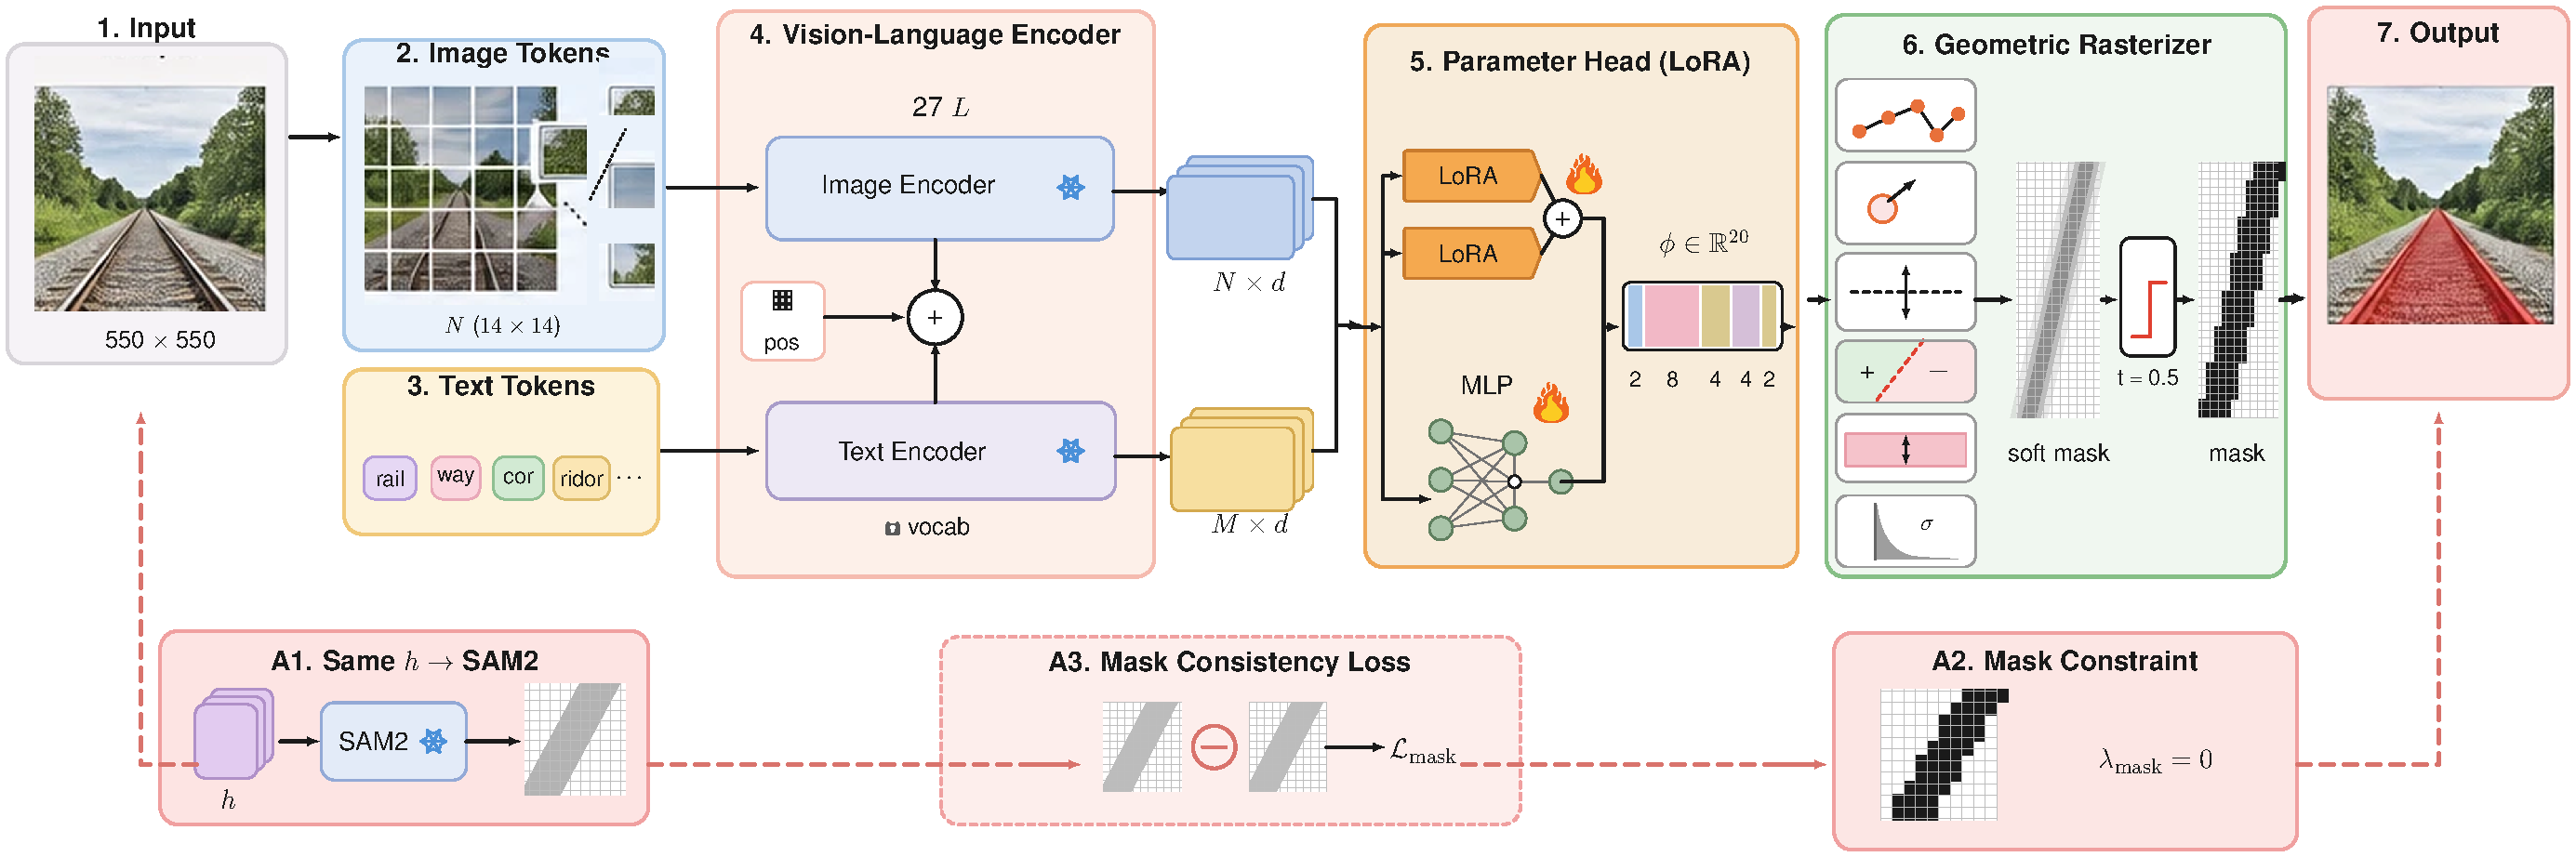
\includegraphics[width=\textwidth]{figures/ecf_framework_vec.pdf}%
\caption{The evaluated forward path, end to end. Panels~1--7: the $550{\times}550$ ego frame and the referring caption enter their token streams, and the frozen vision--language encoder processes both with the vocabulary left unchanged; the corridor head, trained through LoRA adapters on the frozen trunk, reads the first \Seg{} hidden state and emits the $20$ scalars of $\phih$ ($2|8|4|4|2$); the parameter-free rasterizer $\cR$ turns the field into a soft mask, and thresholding at $0.5$ yields the deployed mask. Bottom~row: the same state also reaches frozen SAM2, but its mask loss carries weight zero on this path, so mask supervision enters only through the corridor output (mask-consistency loss $\mathcal{L}_{\mathrm{mask}}$); decoding that state with SAM2 instead is the matched-training control A1 of Table~\ref{tab:ablate}.}
\label{fig:framework}
\end{figure*}

Rail infrastructure inspection relies on precisely localizing a \emph{specific} track among many, given a referring expression such as \emph{``near first from left rail track in frame''}.
This is a referring expression segmentation (RES) task \citep{yu2016refcoco,mao2016refcocog} in an ego-view, corridor-shaped setting: pixels pile up near the camera, thin out toward a vanishing point, and neighboring rails are near-duplicates under the caption.
Modern RES systems couple a multimodal large language model (MLLM) with a mask decoder; Sa2VA \citep{zhang2025sa2va} is the canonical design, where the MLLM emits a \Seg{} token whose hidden state is projected into a frozen SAM2 \citep{ravi2024sam2} decoder.
Off-the-shelf detector-plus-SAM2 pipelines fail badly on this task (gIoU ${\approx}$25--28), consistent with the known difficulty of grounding ordinal phrases like ``first from left'' with open-vocabulary detectors.

Two recent lines of work make the remaining design choice precise.
DeSa2VA \citep{dang2025desa2va} diagnoses three limitations of the shared \Seg{} interface---the token is semantically thin, SAM2 is never trained to read text, and a single hidden state cannot serve as a fine-grained visual prompt---and proposes an \emph{architectural} remedy: linear decoupling of MLLM hidden states, text-derived mask pre-training of SAM2, and mask-level self-feedback.
Independently, parametric lane estimators \citep{tabelini2021polylanenet,feng2022bezierlanenet} show that a corridor in a calibrated ego view is a low-dimensional object: a vanishing-point-anchored centerline plus a width field, not an arbitrary 2-D silhouette.
Rail-specific segmenters make a related simplification: RailSAM \citep{zhang2025railsam} and SMDE-YOLO \citep{lin2026smdeyolo} both produce \emph{class-level} rail masks, which certify that \emph{a} rail is present but do not decide \emph{which} rail an ordinal caption such as ``first from left'' names.
To our knowledge, neither line asks whether a Sa2VA-style \Seg{} token should stop talking to SAM2 altogether and instead emit that low-dimensional corridor, rasterized differentiably to a mask.

We ask that question.
After language has selected \emph{which} rail, the mask SAM2 is asked to produce is the region of a perspective corridor whose shape is more compactly described by parameters than by pixels, so our key idea is an Ego-Corridor Field ($\ECF$): the same \Seg{} hidden state is mapped by a ParamHead to $\phih \in \mathbb{R}^{20}$, and a differentiable rasterizer $\cR(\phih)$ produces the RES mask.
SAM2 remains in the codebase but is \emph{bypassed} on the training and inference path that we evaluate.
The rasterizer is part of the paradigm, not an optional post-process: if the same trained embeddings are fed to SAM2, the mask collapses (to $2.43$ gIoU), and if the raster mask loss is removed, the high-IoU rate drops sharply ($\PrAt{0.7}$ $87.98\to54.81$) while the mean falls only to $69.31$ gIoU.

Concretely, we train InternVL3-2B with LoRA and a 20-D ParamHead on the first \Seg{} token, using BCE+Dice on $\cR(\phih)$ against FIRC2234 masks plus a parameter loss on geometry-derived $\phih^{gt}$.
The training set is the original 1664 frames plus their horizontal flips (captions and $\phih^{gt}$ transformed to match the mirrored geometry), while val/test stay on original images; we evaluate only fp32 ECF-native decoding.
Our contributions are:

\begin{itemize}
\item \textbf{A carrier-level answer to DeSa2VA's sparse-\Seg{} diagnosis.} Without decoupling SAM2, we stop using SAM2 as the mask decoder and let \Seg{} predict a low-dimensional corridor parameterization.
\item \textbf{A differentiable rasterization closed loop.} $\cR$ maps $\phih$ to a soft mask; A1 (same weights, SAM2 decode) and A2 (no raster mask loss) are the falsifiers that show the loop is load-bearing.
\item \textbf{Same-protocol performance against the off-the-shelf reference set.} On FIRC2234 test (208 frames, fp32), ECF (gIoU 80.67) outperforms GroundingDINO+SAM2 (28.18) and Qwen2.5-VL-7B+SAM2 (25.60) by 2.9--3.2$\times$, and pretrained Sa2VA (14.32) by 5.6$\times$. These three off-the-shelf systems are the only reference rows of Table~\ref{tab:main}. The same checkpoint transfers, eval-only, to RailSem19-EgoPair and RailBench 1L1R. A SAM2 zero-shot oracle, reported in the supplementary material only, is not deployable and is not a competitor.
\end{itemize}

\paragraph{What is and is not compared.}
FIRC2234 is a new benchmark introduced here; to our knowledge, no published method has been trained on it, so the comparison is drawn against off-the-shelf systems applied without task-specific adaptation (Section~\ref{sec:setup}).
Those rows quantify how far an untrained generalist is from solving ordinal rail selection.
The control that isolates the carrier under matched training is A1 (Section~\ref{sec:ablate}): the very same ECF LoRA and ParamHead weights, decoded by SAM2 instead of $\cR$, fall to near-zero IoU, which counters the trivial reading that the masks come from the language backbone, and Section~\ref{sec:discussion} places this control next to DeSa2VA's encoder-side treatment.
Figure~\ref{fig:framework} is the evaluated forward path.

The rest of this paper is organized as follows.
Section~\ref{sec:related} positions the work against DeSa2VA, parametric lanes, and RES;
Section~\ref{sec:method} describes $\phih$, the ParamHead, and $\cR$;
Section~\ref{sec:exp} reports the protocol, the reference set, and the ablations;
Section~\ref{sec:discussion} discusses how a geometric carrier relates to token decoupling;
and Section~\ref{sec:conclusion} concludes.
